\subsection{Grayscale to RGB}
For our project we were provided with three SEVIRI visible channels: VIS 0.6, VIS 0.8, IR 1.6 %(reference p7 in summary of kit doc sent by Frazer) 
from METSAT 9. Channel wavelengths were centred on 0.635 $\mu$m [0.56-0.71 $\mu$m], 0.81 $\mu$m [0.74-0.88 $\mu$m] and 1.64 $\mu$m [1.50-1.78 $\mu$m] respectively, (p9) where the bracketed ranges show the spectral bandwidths of each channel. 
\par The first step required for analysis of this data was the visualisation of the channels provided, both individually and as an RGB image. The construction of an RGB image requires three channels, one representing the red spectra, one for the green and the final one for the blue. The channels given were not provided in this format and we therefore had to select how to stack our three channels in place of the red, green and blue channels in a traditional image. Approximate wavelength ranges for the visible spectrum are given in nanometres by Red: 780 - 622, Orange: 622 - 597, Yellow: 597 - 577, Green: 577 - 492, Blue: 492 - 455 and Violet: 455 - 390. %(reference website url https://www.livephysics.com/physical-constants/optics-pc/wavelength-colors/, can use better reference than if found I just picked one that seemed reliable?). 
From these values we determined that the nearest approximation of these channels with the 3 channels we have access to is Red: IR 1.6, Green: VIS 0.8, and Blue: VIS 0.6. 
\par For a desired datetime we created a function that searched the images for the corresponding channel files, and subsequently selected and read them into numpy arrays. These three arrays were then stacked in the order defined above, before being displayed as an RGB image as shown in Fig.~\ref{}. To obtain a more accurate RGB image, a weighting can be added to each channels values to adjust for the difference in channel wavelength values. 
\subsection{Cloud Removal}
 Before analysis can be done on satellite data to track changes in vegetation, crop growth, deforestation and sea temperature etc, the cloud cover obscuring the surface must first be taken into account and removed. There are a number of ways of doing this, a couple of which we explored and compared in our project. 
\subsubsection{Averaging Pixel Values}
 One of the simplest but most ineffectual ways of obtaining a cloud free image is to calculate an average image using multiple images centred over the same area on the Earth's surface. This works by assuming that there are a greater number of images with cloud free areas than cloudy ones, and that these cloud free pixels will reduce the influence of the cloudy pixels in the final image. The effectiveness of this technique very much depends on the ratio of cloud free days to covered ones and may also introduce cloudy pixels to areas that were previously cloud free. To illustrate this we plotted an averaged image by stacking multiple images together in four dimensions and averaging over the pixel values for each RGB channel as shown in Fig.~\ref{}. This image demonstrates why it is preferable to use other methods of cloud cover removal before further analysis of the image, as the image obtained still contains areas of cloud cover that prevent easy analysis of the terrain.
% Did we just straight up average over the images ? I can do if we haven't and we want it in the report to demonstrate why thresholding and masking is necessary and why we can't just average pixels over multiple days. 
\subsubsection{Thresholding Via Inspection}
 A common method of cloud cover removal makes use of thresholding to determine the cloudy and non-cloudy pixels. Thresholding allows an image to be split into two or more regions based on given threshold values. It works by setting all values above the chosen threshold to one value and all values below the threshold value to another, either 1 or 0 depending on which section of the image is desired as shown in Eq.~\ref{eq:thresh}.
 \begin{equation}\label{eq:thresh}
     g(x,y)=\Big\{\begin{matrix}
1 & if~f(x,y)~>~ T\\
0 & otherwise
\end{matrix}
 \end{equation}
 In the case of multiple threshold values it is the ranges between these values that have the same value assigned to them. Thresholding an image results in a binary image that can then be used as a mask to select the desired parts of an image and hide other areas. The differing cloud and surface level pixel values in the VIS 0.6 and VIS 0.8 channels meant that we were able to set threshold values to create masks to cover (and therefore remove) the cloud cover from our images. Due to the variation in the pixel values across the Earth's surface depending on latitude and longitude, a smaller area of 200x200 pixels was selected upon which to apply this cloud removal method. The threshold values were initially chosen via inspection of the RGB pixel values of the cloudy pixels in the plotted RGB image, and were further adjusted once the masks were applied. This was done by setting threshold ranges for each RGB channel and creating a two dimensional mask array of 1s,  in which the pixel's were set to 0 if the corresponding pixel values fell within the threshold ranges in all three channels. A three dimensional mask was then created by stacking three copies of this same two dimensional mask, which was then multiplied element wise with the RGB image channels to produce a cloud free image as shown in Fig.~\ref{}. 
 
\subsubsection{Otsu's Method for Thresholding}

As can be seen in Fig.~\ref{} although the threshold values chosen were successful at removing most of the cloud cover there are still areas where cloudy pixels are present and better threshold values are required to remove these. There are multiple methods that can analytically determine "optimum" threshold values for image segmentation based off of different definitions of "goodness". One such method is Otsu's method. This is an automatic global thresholding technique that calculates the optimum threshold values for each image so that the measure of separability is maximised and the spread of pixel levels is minimised for the foreground (cloudy) and background (cloud free) pixels. Such algorithms usually consist of the computation of optimum threshold values followed by the replacement of image pixels by 0 and 1 depending on where they fall in relation to the threshold value/s. This thresholded mask can then be applied to the original image to remove the unwanted pixel values.

\par
The interpixel variance (the measure by which separability is computed) for each threshold value can be calculated by going through the steps shown in Fig.~\ref{fig:flowchart}. The equation used to calculate this is given by Eq.~\ref{eq:interpixvar}

\begin{equation}\label{eq:interpixvar}
\sigma_{B}^{2}(k)=\frac{\left(m_{G} P_{1}(k)-m(k)\right)^{2}}{P_{1}(k)\left(1-P_{1}(k)\right)}
\end{equation}

where $\sigma_{B}^{2}(k)$ is the interpixel variance for threshold value $k$, $m_G$ is the global mean of the pixel values, $P_{1}(k)$ is the cumulative probability and $m(k)$ is the cumulative mean of the pixel values up to the threshold pixel value $k$.

\par
The first step is this calculation was to plot a histogram of the distribution of the pixel values in the image, similar to the one seen in Fig.~\ref{}. Once the histogram of the pixel values had been plotted the frequency of each pixel value was then used to calculate the probability of occurrence of each value using Eq.~\ref{eq:prob}

\begin{equation}\label{eq:prob}
p_{i}=\frac{n_{i}}{N}
\end{equation}

where $p_{i}$ is the probability of occurrence of pixel value $i$, $n_{i}$ is the frequency of occurrence, and $N$ is the total number of pixels.

\par
The cumulative probability for each threshold value, otherwise expressed as the probablity that a pixel will either be equal to or less than the threshold value, was subsequently calculated from Eq.~\ref{eq:probcum}

\begin{equation}\label{eq:probcum}
P_{1}(k)=\sum_{i=0}^{k} p_{i}
\end{equation}

\begin{wrapfigure}{r}{0.5\textwidth}
%\centering
    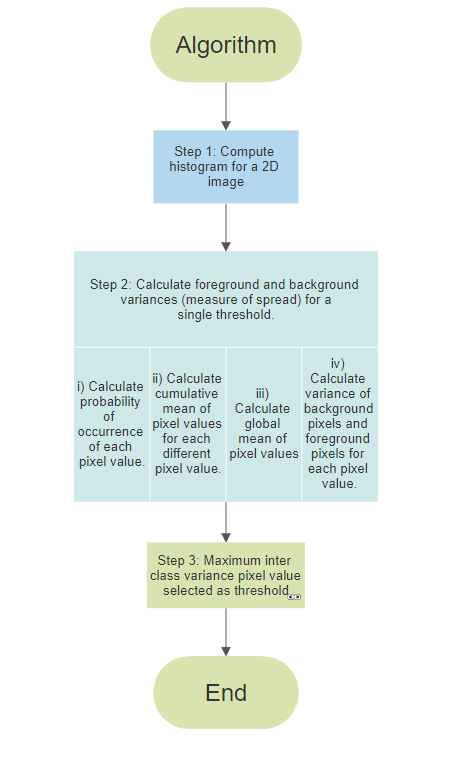
\includegraphics[width=0.6\textwidth]{flowchart_otsu.png}
    \caption{\label{fig:flowchart}}
\end{wrapfigure}

with the cumulative mean being subsequently calculated from Eq.~\ref{eq:cummean}.

\begin{equation}\label{eq:cummean}
m(k)=\sum_{i=0}^{k} i p_{i}
\end{equation}

where $i$ is the pixel value.

Using the equations introduced above we calculated the inter-class variance for each threshold value and saved the values into an array where the index of the element corresponded to the pixel threshold values. From this we selected the pixel index value of a peak in the inter-class variance array as the optimum threshold value for cloud and terrain separation. These threshold values were then used as previously (when thresholding via inspection) to create masks which were then multiplied element wise with the RGB image to hide the cloudy pixels.
This was done for multiple different areas over the Earth's surface to test the effectiveness of the threshold values selected via both inspection and the computation of the separability measure given by Eq.~\ref{eq:sepm}.

\begin{equation}\label{eq:sepm}
    \eta = \frac{\sigma_{B,max}^{2}}{\sigma_{G}^{2}}
\end{equation}

where $\eta$ is the separability measure, $\sigma_{B,max}^{2}$ is the maximum interpixel variance (the interpixel variance of the selected threshold value) and $\sigma_{G}^{2}$ is the interpixel variance of all the pixels. The closer the separability measure is to 1, the better the chosen threshold value is as maximising the interpixel variance.

For selection areas that straddled both land and sea pixels, the automatically calculated thresholds obtained using Otsu's algorithm grouped land and cloud values together as opposed to land and sea as shown in Fig.~\ref{}. %This occurred due to there being a greater distinction between the land and water pixel values than the land and cloud. 
To overcome this hurdle in our automatic cloud removal algorithm we considered a couple of possible options. One of these was the use of a landmask provided to us alongside the channel images, which could be used to hide the sea and/or land pixels. To enable use of this mask we adjusted our function so that if an area was specified to contain both land and sea, it would select the desired part of the mask and apply it first to the sea and then subsequently to the land. The new masked images then separately went through Otsu's algorithm for optimum threshold value detection and had further masks applied to them to remove the cloudy pixels. The channels used for the determination of threshold values were VIS 0.6 for land pixels and VIS 0.8 for sea pixels as recommended by many authors \cite{}. 
% Francisco Javier Batllesa, Joaqu´ın Alonsob, Gabriel L´opez. Cloud cover forecasting from METEOSAT data. url: 10.1016/j.egypro.2014.10.122.
The result of these separate threshold value determinations enabled better distinctions to be made between land and cloud pixels as shown in Fig.~\ref{} and Fig.~\ref{}

\subsection{Average Pixel Replacement}

Removal of the cloudy pixel values resulted in images with empty pixel values, which although removed the influence of cloud cover from further analysis also didn't provide a better understanding of the terrain which the clouds were covering. In an attempt to retrieve pixel values similar to the ones that would have been present were it not for the cloud cover, we calculated the average pixel value for each cloud free pixel over the period of one month and combined them to form an averaged cloud free image of the terrain for a desired month. These average monthly pixel values can then be substituted back into the empty pixel values for each image in the month to obtain a more accurate cloud free image which can then be used for further terrain analysis.

\subsection{Change in Percentage Cloud Cover}

The generated cloud cover masks were also used to determine the percentage cloud cover present in an image, as well as for cloud removal. This was done by counting the number of cloudy pixels and dividing by the total number of pixels in the image. The percentage cloud cover for a selected area of the Earth's surface was then plotted against time across multiple months as shown in Fig.~\ref{}

\subsection{Normalised Difference Vegetation Index (NDVI)}
Our newly cloud free images allow us to conduct further analysis of the Earth's surface. An example of this is the classification and monitoring of surface vegetation using the Normalised Difference Vegetation Index (NDVI) which was initially used as a measure of green biomass and is now widely used as an indicator for crop and vegetation monitoring. NDVI is a measure of the density of vegetation on a patch of land, measuring the difference between the near-infrared and red reflectances. This value is unitless,  always falls between -1 and +1 and can be calculated from Eq.~\ref{eq:ndvi}

\begin{equation}\label{eq:ndvi}
    NDVI = \frac{R_{NIR}-R_{VIS}}{R_{NIR}+R_{VIS}}
\end{equation}

where $R_{NIR}$ is the near-infrared reflectance and $R_{VIS}$ is the red reflectance.
Healthy green vegetation is normally indicated by high positive NDVI values, while vegetation free surfaces such as water, ice, snow and clouds tend to have negative NDVI values, and deserts and bare terrain have values close to 0.

The NDVI values for our pixels were calculated by applying Eq.~\ref{eq:ndvi} to each pixel using the IR 1.6 channel in the place of the near-infrared channel and the VIS 0.6 channel for the visible light channel. A plot of the different NDVI values calculated can be seen in Fig.~\ref{}.

\par Snow cover can also be identified using a similar index, the normalised difference snow index (NDSI), given by Eq.~\ref{eq:ndsi}

\begin{equation}\label{eq:ndsi}
    NDSI = \frac{R_{0.66}-R_{1.6}}{R_{0.66}+R_{1.6}}
\end{equation}

where $R_{0.66}$ is the reflectance of visible wavelengths at 0.66 $\mu$m, and $R_{1.6}$ is the reflectance of wavelengths at 1.6 $\mu$m.

% A measure of




